\documentclass{article}

\usepackage{fullpage}
\usepackage[round]{natbib}
\usepackage{multirow}
\usepackage{booktabs}
\usepackage{tabularx}
\usepackage{graphicx}
\usepackage{float}
\usepackage{hyperref}
\usepackage{array}

\input{../Comments}
\input{../Common}

\title{User Guide\\\progname}

\author{\authname}

\date{}

\begin{document}

\begin{table}[hp]
\caption{Revision History} \label{TblRevisionHistory}
\begin{tabularx}{\textwidth}{llX}
\toprule
\textbf{Date} & \textbf{Developer(s)} & \textbf{Change}\\
\midrule
March 31 2023 & Jared Bentvelsen, Matthew McCracken & Description of changes\\
\bottomrule
\end{tabularx}
\end{table}

\newpage

\maketitle

\tableofcontents

\section{Introduction}

This document serves to go over the usage details of the Olympian application, allowing any potential reader to familiarize themselves with all functionality.

\section{Reference Material}

This section records information for easy reference.

\subsection{Definitions}

\renewcommand{\arraystretch}{1.2}
\begin{tabular}{|l|p{1\linewidth}|}
  \toprule		
  \textbf{symbol} & \textbf{description}\\
  \midrule   
  Exercise & Exercises are individual movements that people will do during a workout in order to develop the strength of certain muscle groups.\\
  Workout & Workouts are collections of Exercises strung together in order to build one cohesive trip to the gym. Often workouts will be a collection of exercises that target one specific muscle group such as a chest day.\\
  Program & A Program is a series of workouts that a user adds to their collection. A user will follow the schedule of a program to do workouts on selected days.\\
  \bottomrule
\end{tabular}\\

\section{Installation}

\subsection{Database Setup}

Steps to setup Database:
\begin{enumerate}
    \item Download the pgAdmin 4 postgres SQL tool
    \item Setup a database called olympian
\end{enumerate}

\subsection{Git Repo Setup}
    Clone the repo and navigate to `src/hermes`.\\
    Create a .env file in hermes and fill it with the following data:

    \begin{verbatim}
        PORT=4000
        DATABASE_URL="{$YOUR_DATABASE_USER_HERE}://postgres:{$YOUR_DATABASE_PASSWORD_HERE}@localhost:5432/olympian?schema=public"
        JWT_SECRET={$YOUR_JWT_SECRET_HERE}
    \end{verbatim}

    Run:
    \begin{verbatim}
    npm i && npm run migrate && npm run generate && npm run dev
    \end{verbatim}

    navigate to `src/athena`. 
    
    Create a .env file in athena and fill it with the following data:

    \begin{verbatim}
        IP_ADDRESS={$YOUR_IP_ADDRESS_HERE}
        PORT=4000
    \end{verbatim}

    Run:
    \begin{verbatim}
    npm i && npm run gen
    \end{verbatim}

\section{Usage}

\subsection{Starting the application}

In a terminal in the src/hermes folder, run:
    \begin{verbatim}
    npm run dev
    \end{verbatim}

Wait for the following message:
    \begin{verbatim}
    Server ready at port http://localhost:4000/graphql
    \end{verbatim}

In a WSL terminal in the src/athena folder, run:
    \begin{verbatim}
    npm run start
    \end{verbatim}

Wait for a QR code to appear in the terminal. Scan the QR code using the Expo application and wait for the app to bundle and open.\\
For first time users, the app will open to the Landing Screen shown in Figure \ref{FigLanding}:
\begin{figure}[H]
    \centering
    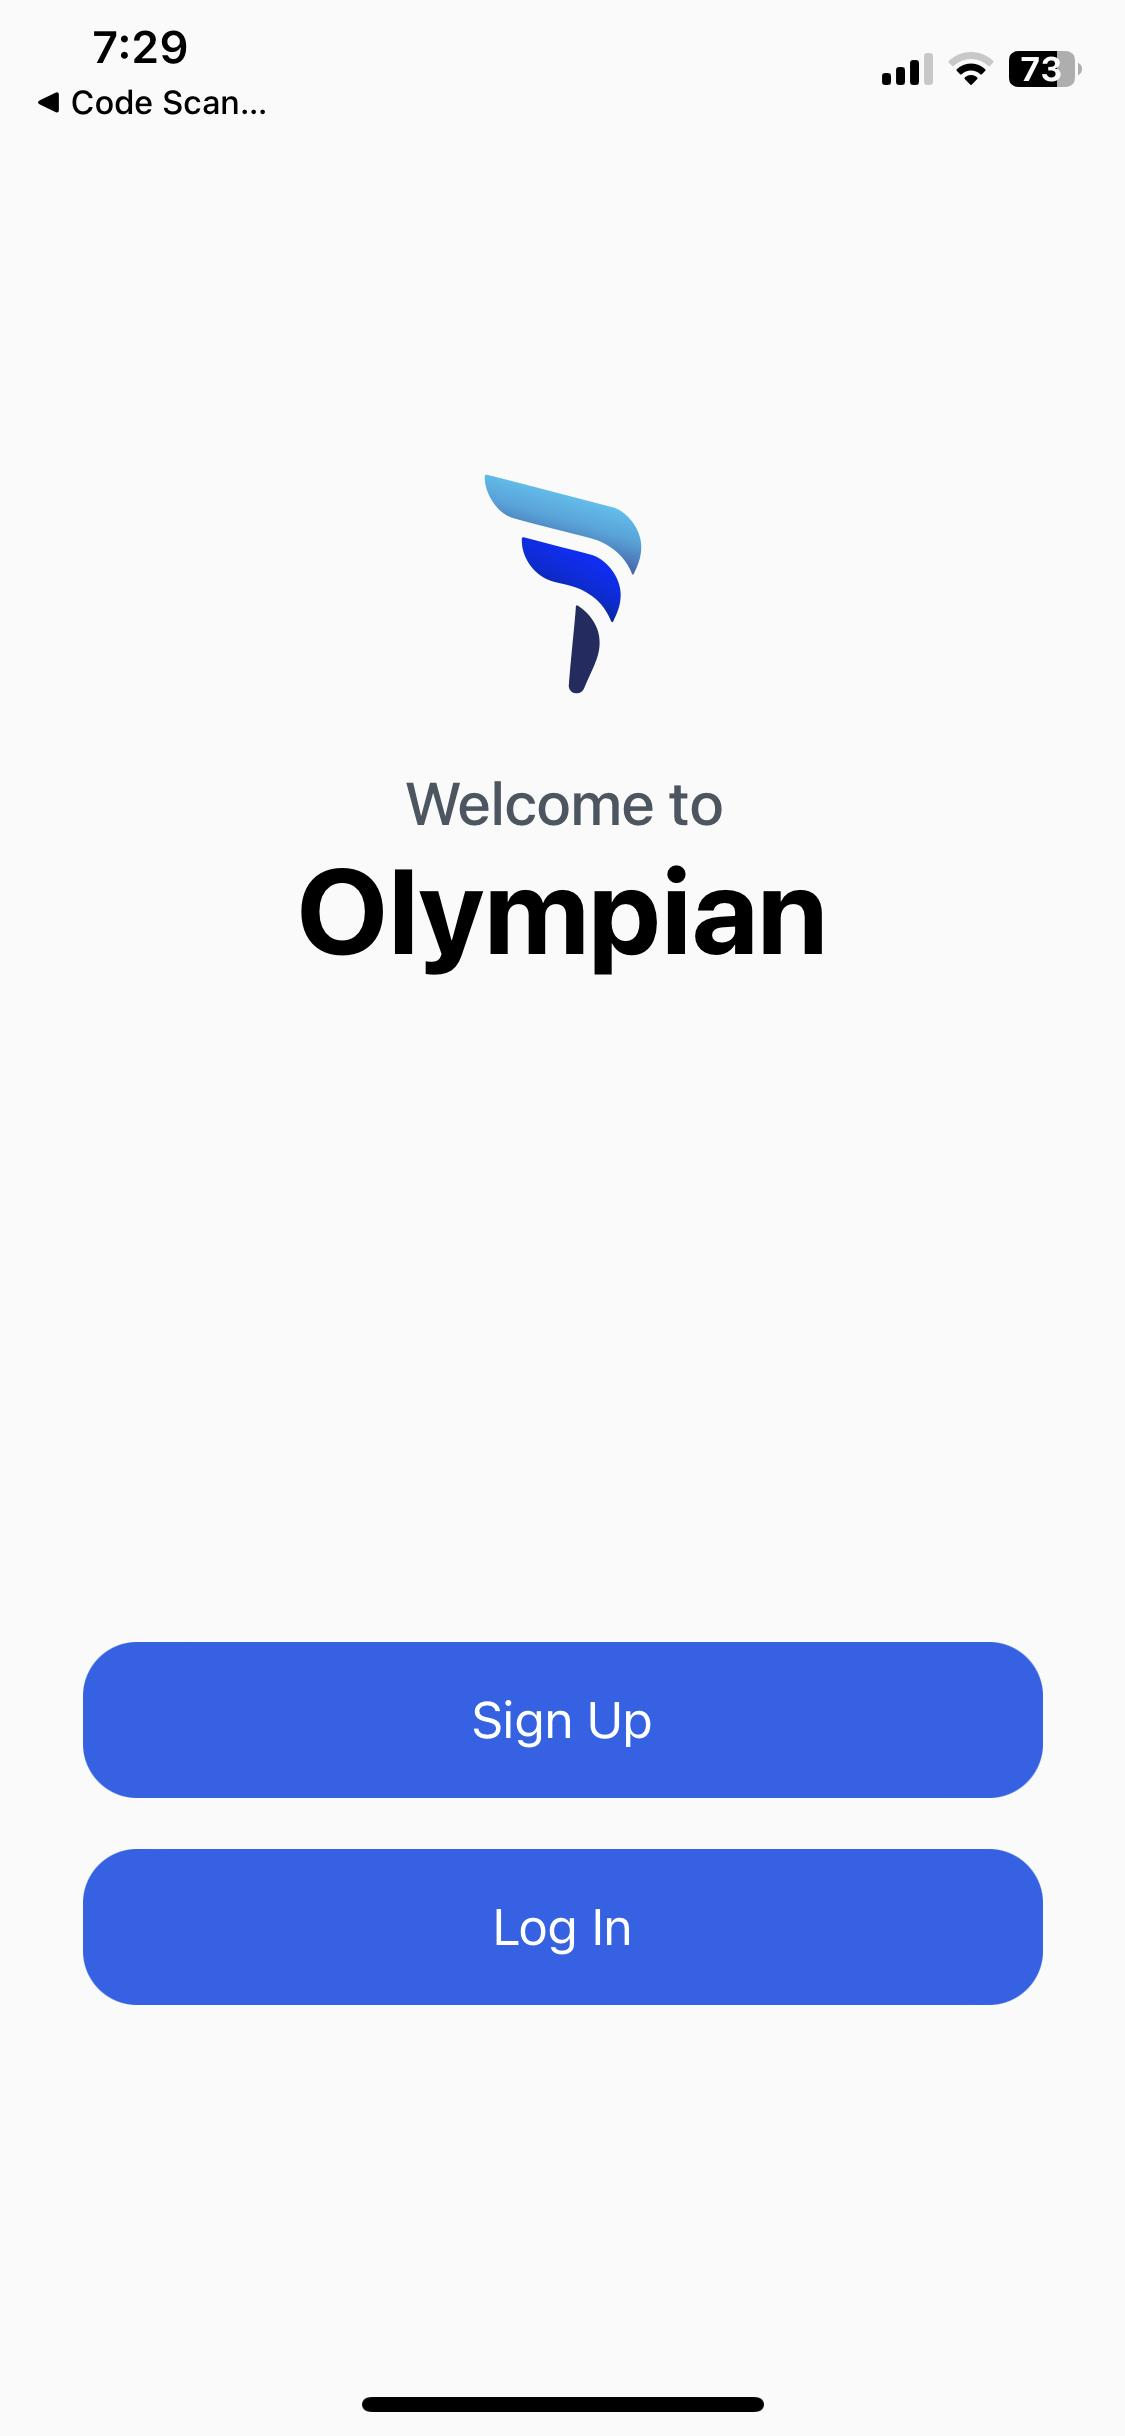
\includegraphics[height=0.6\textwidth]{imgs/Landing.jpg}
    \caption{Landing Screen}
    \label{FigLanding}
    \end{figure}


\subsection{Using the Application}

\subsubsection{Sign Up}

From the screen shown in Figure \ref{FigLanding} users will enter their name, email, and intended username and password. If any of these details do not meet our criteria the user will be informed of the error and prevent from progressing.\\
After entering all information then a new user is created in the database and the user is redirected to the Log In Screen.

\subsubsection{Login}

Users must enter in the information of a user that exists within the database in order to access their account. When they do this, they will be redirected to the app home screen. For first time users this will look like the screen shown in Figure \ref{FigHomeScreen} 

\begin{figure}[H]
    \centering
    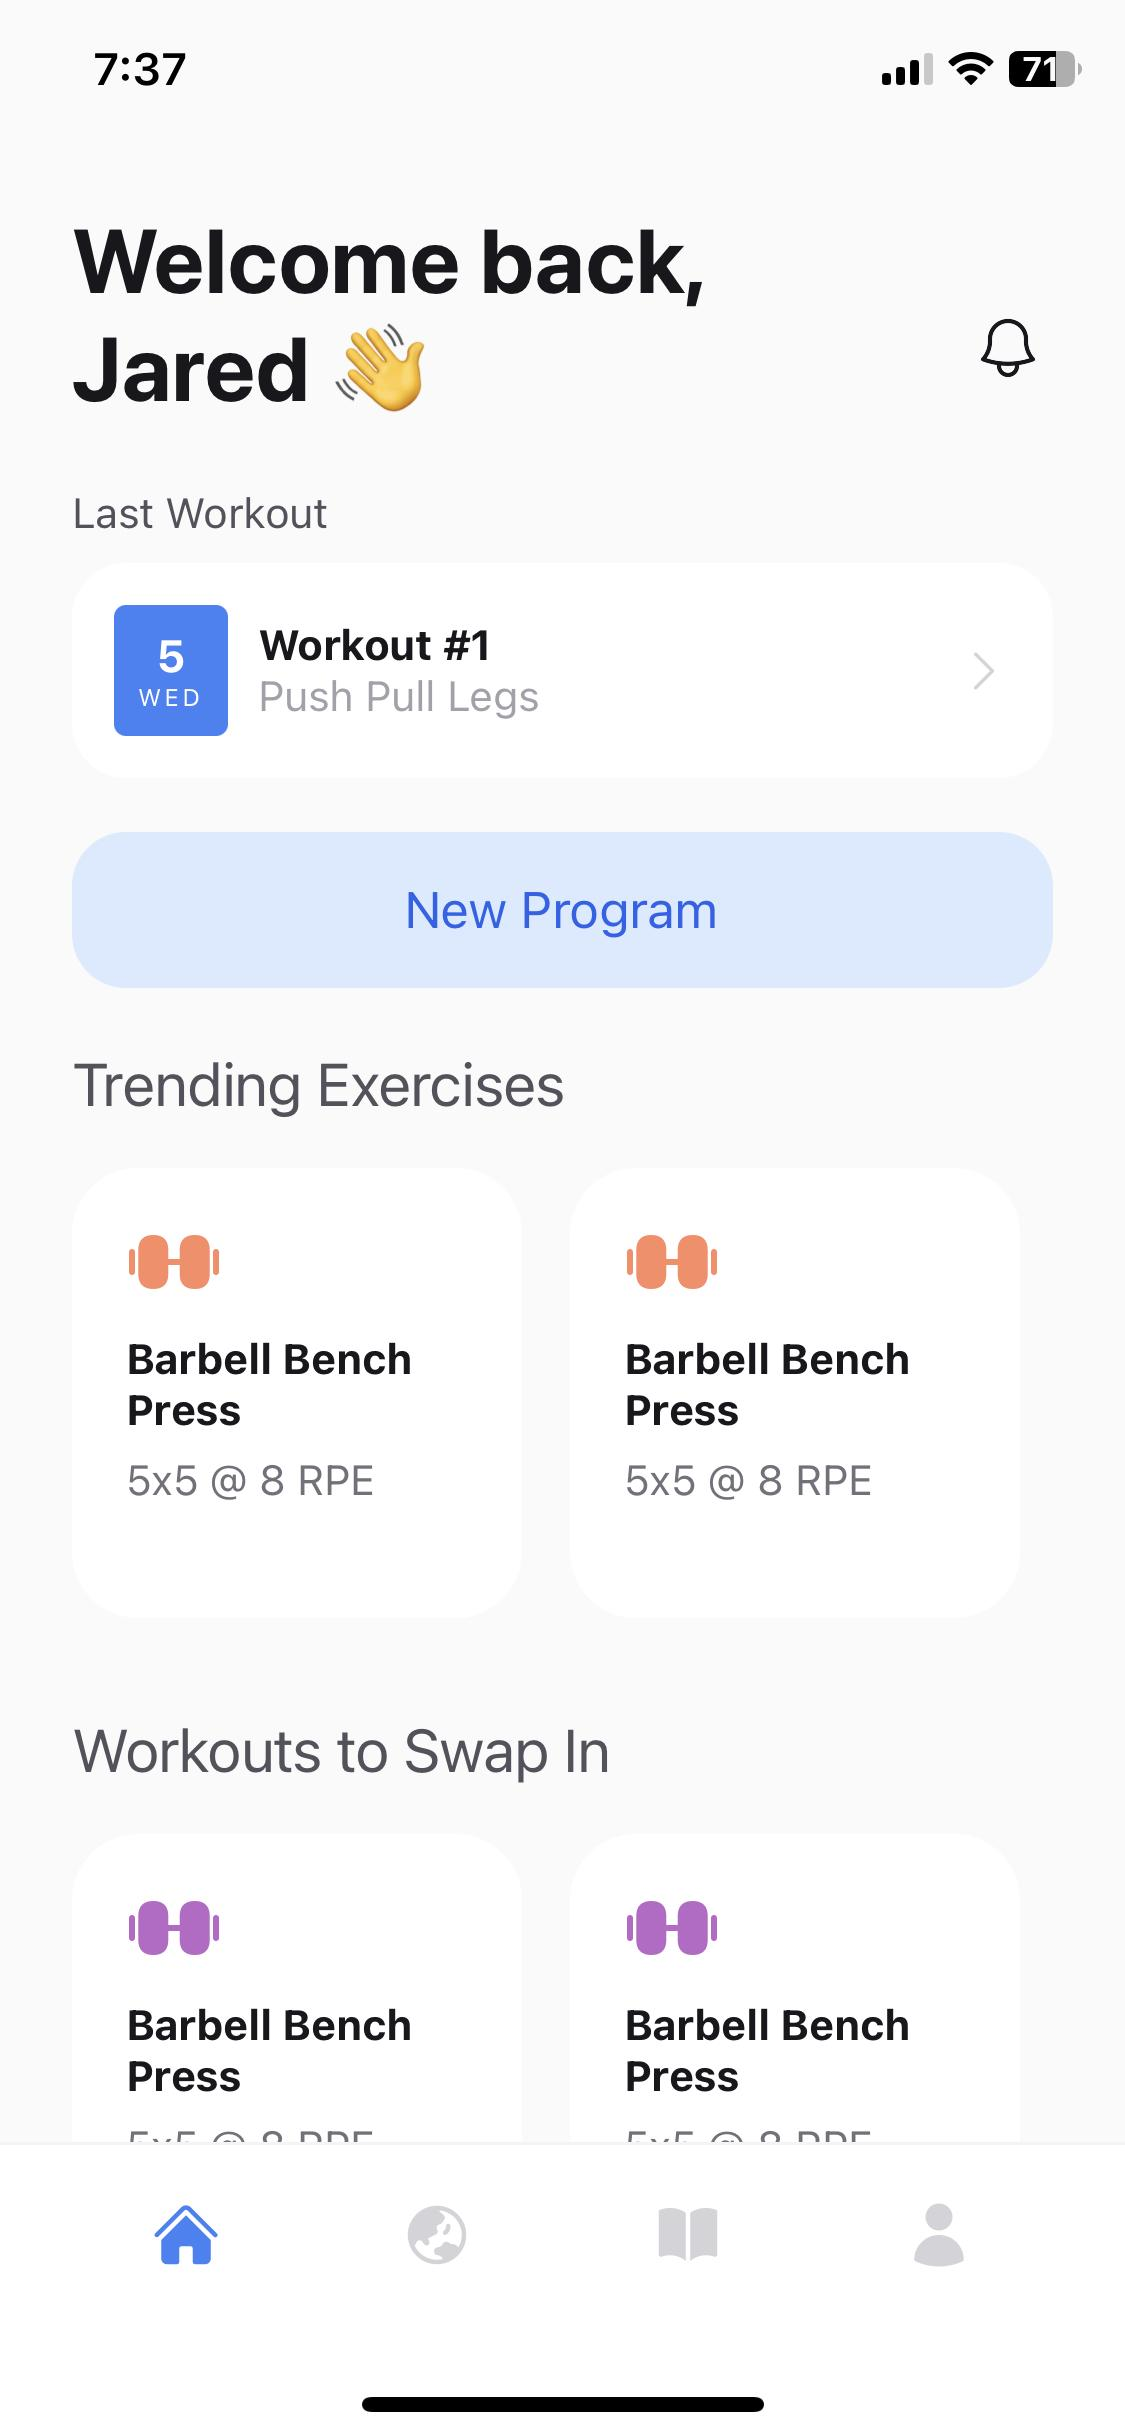
\includegraphics[height=0.6\textwidth]{imgs/LastWorkout.jpg}
    \caption{Home Screen}
    \label{FigHomeScreen}
    \end{figure}

\subsubsection{Program Creation}

From the home screen as shown in \ref{FigHomeScreen} users can select 'Add Program' or select 'Get Started' and add a program in order to access the program creation page.\\
Users will select a name, the publicity settings for their created workout, and any tags that they want applied. They can then see the overview of their created program on the program screen.\\
When on the program screen as shown in \ref{FigProgramScreen} users can select what icon they want and begin adding workouts to their program.

\begin{figure}[H]
    \centering
    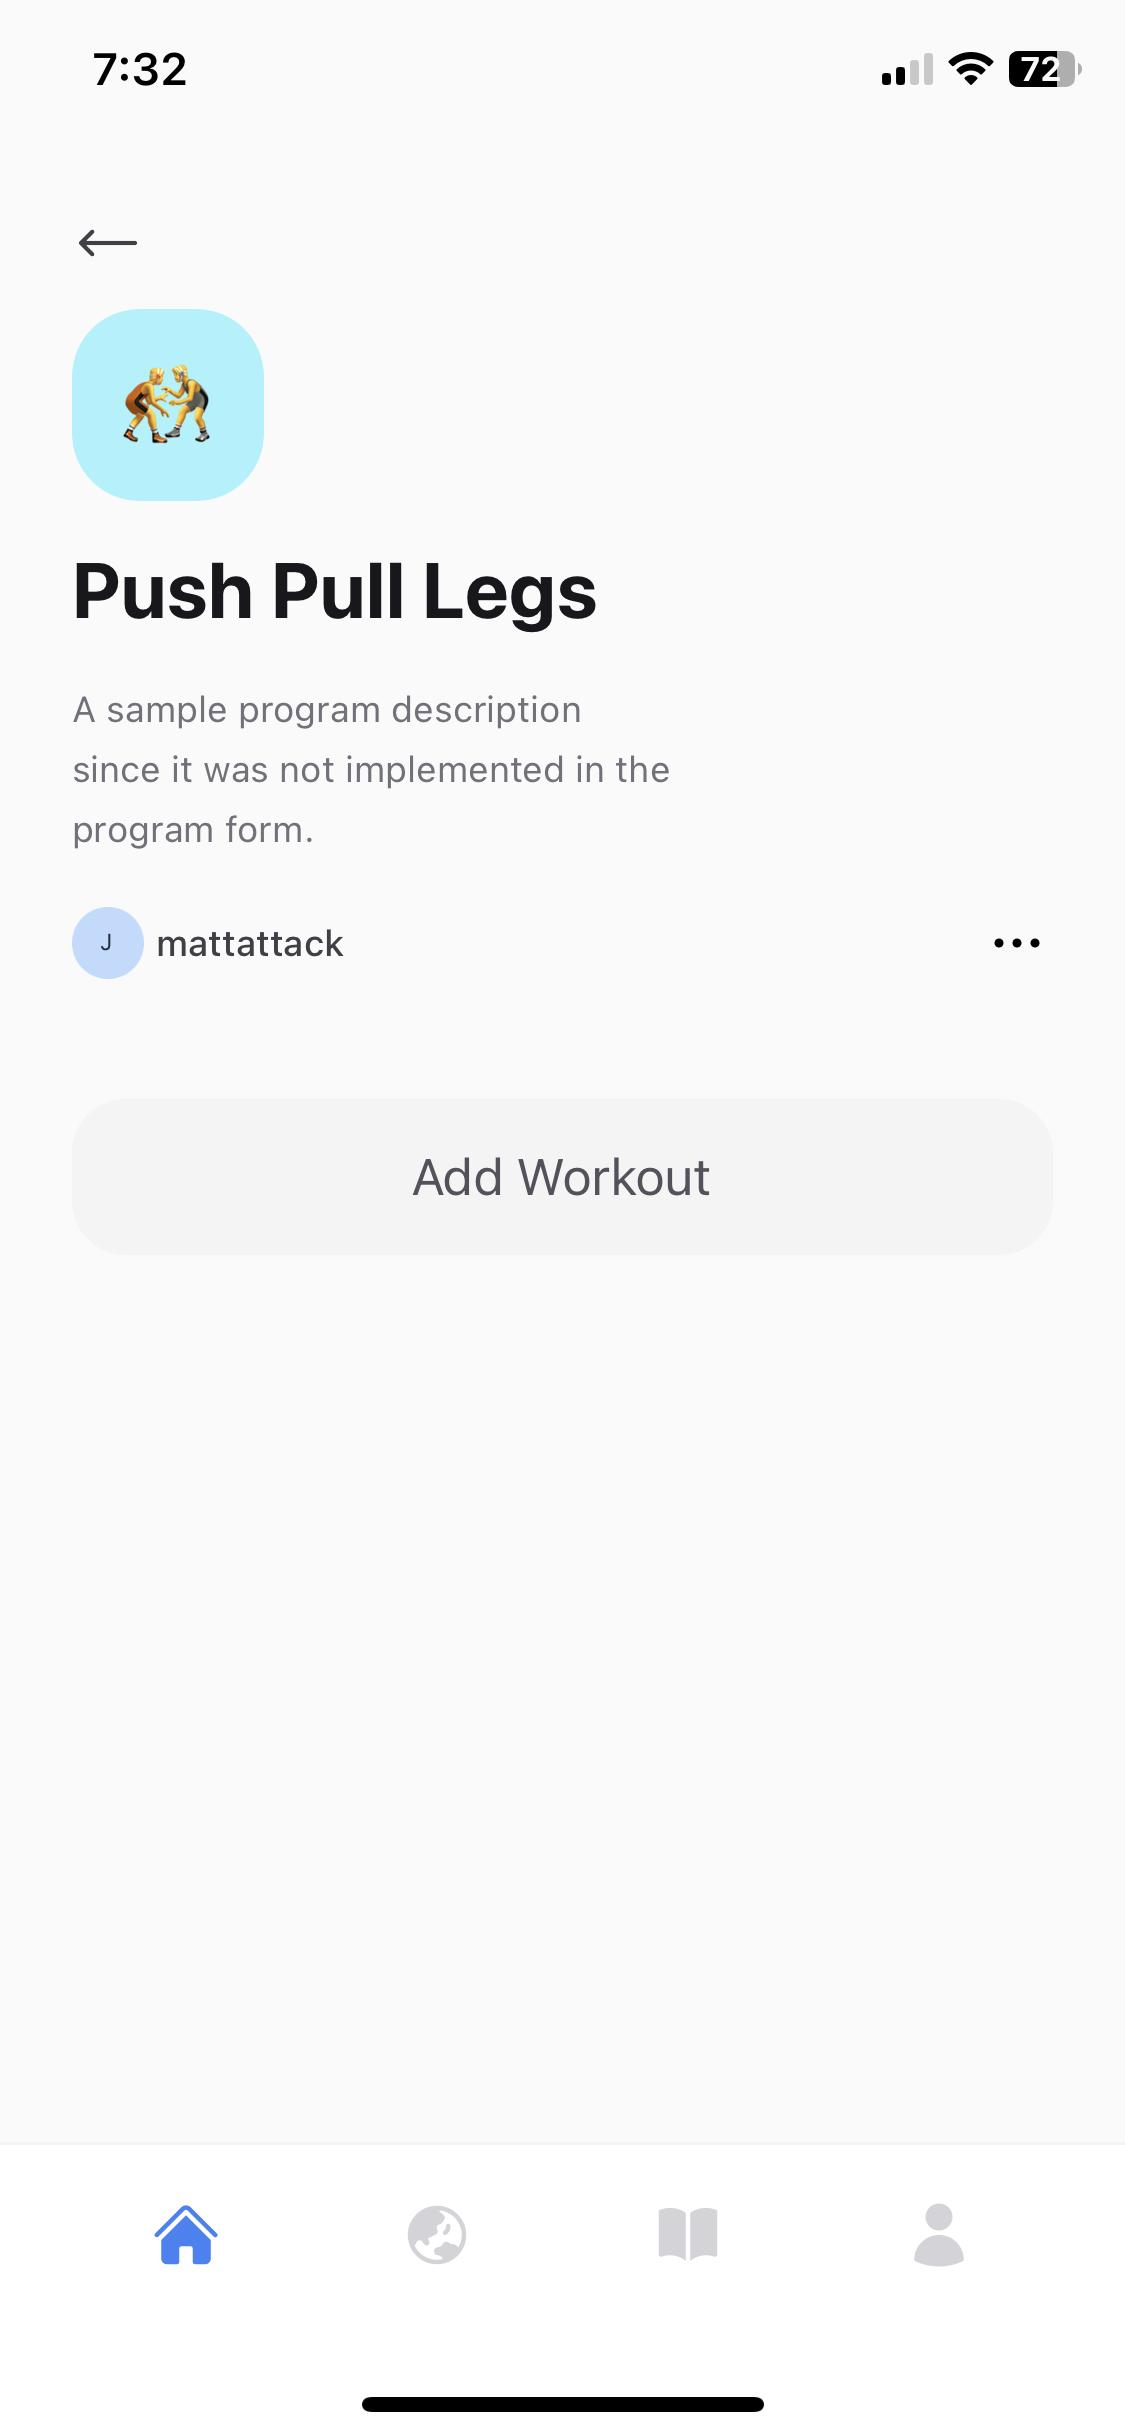
\includegraphics[height=0.6\textwidth]{imgs/Programs.jpg}
    \caption{Program Screen}
    \label{FigProgramScreen}
    \end{figure}

\subsubsection{Workout Addition}

After pressing 'Add Workout' users will be taken to the 'Edit Workout' page as shown in \ref{FigEditWorkout}. From here, users can edit the name of their workouts and add exercises by pressing 'Add Exercise'.\\

\begin{figure}[H]
    \centering
    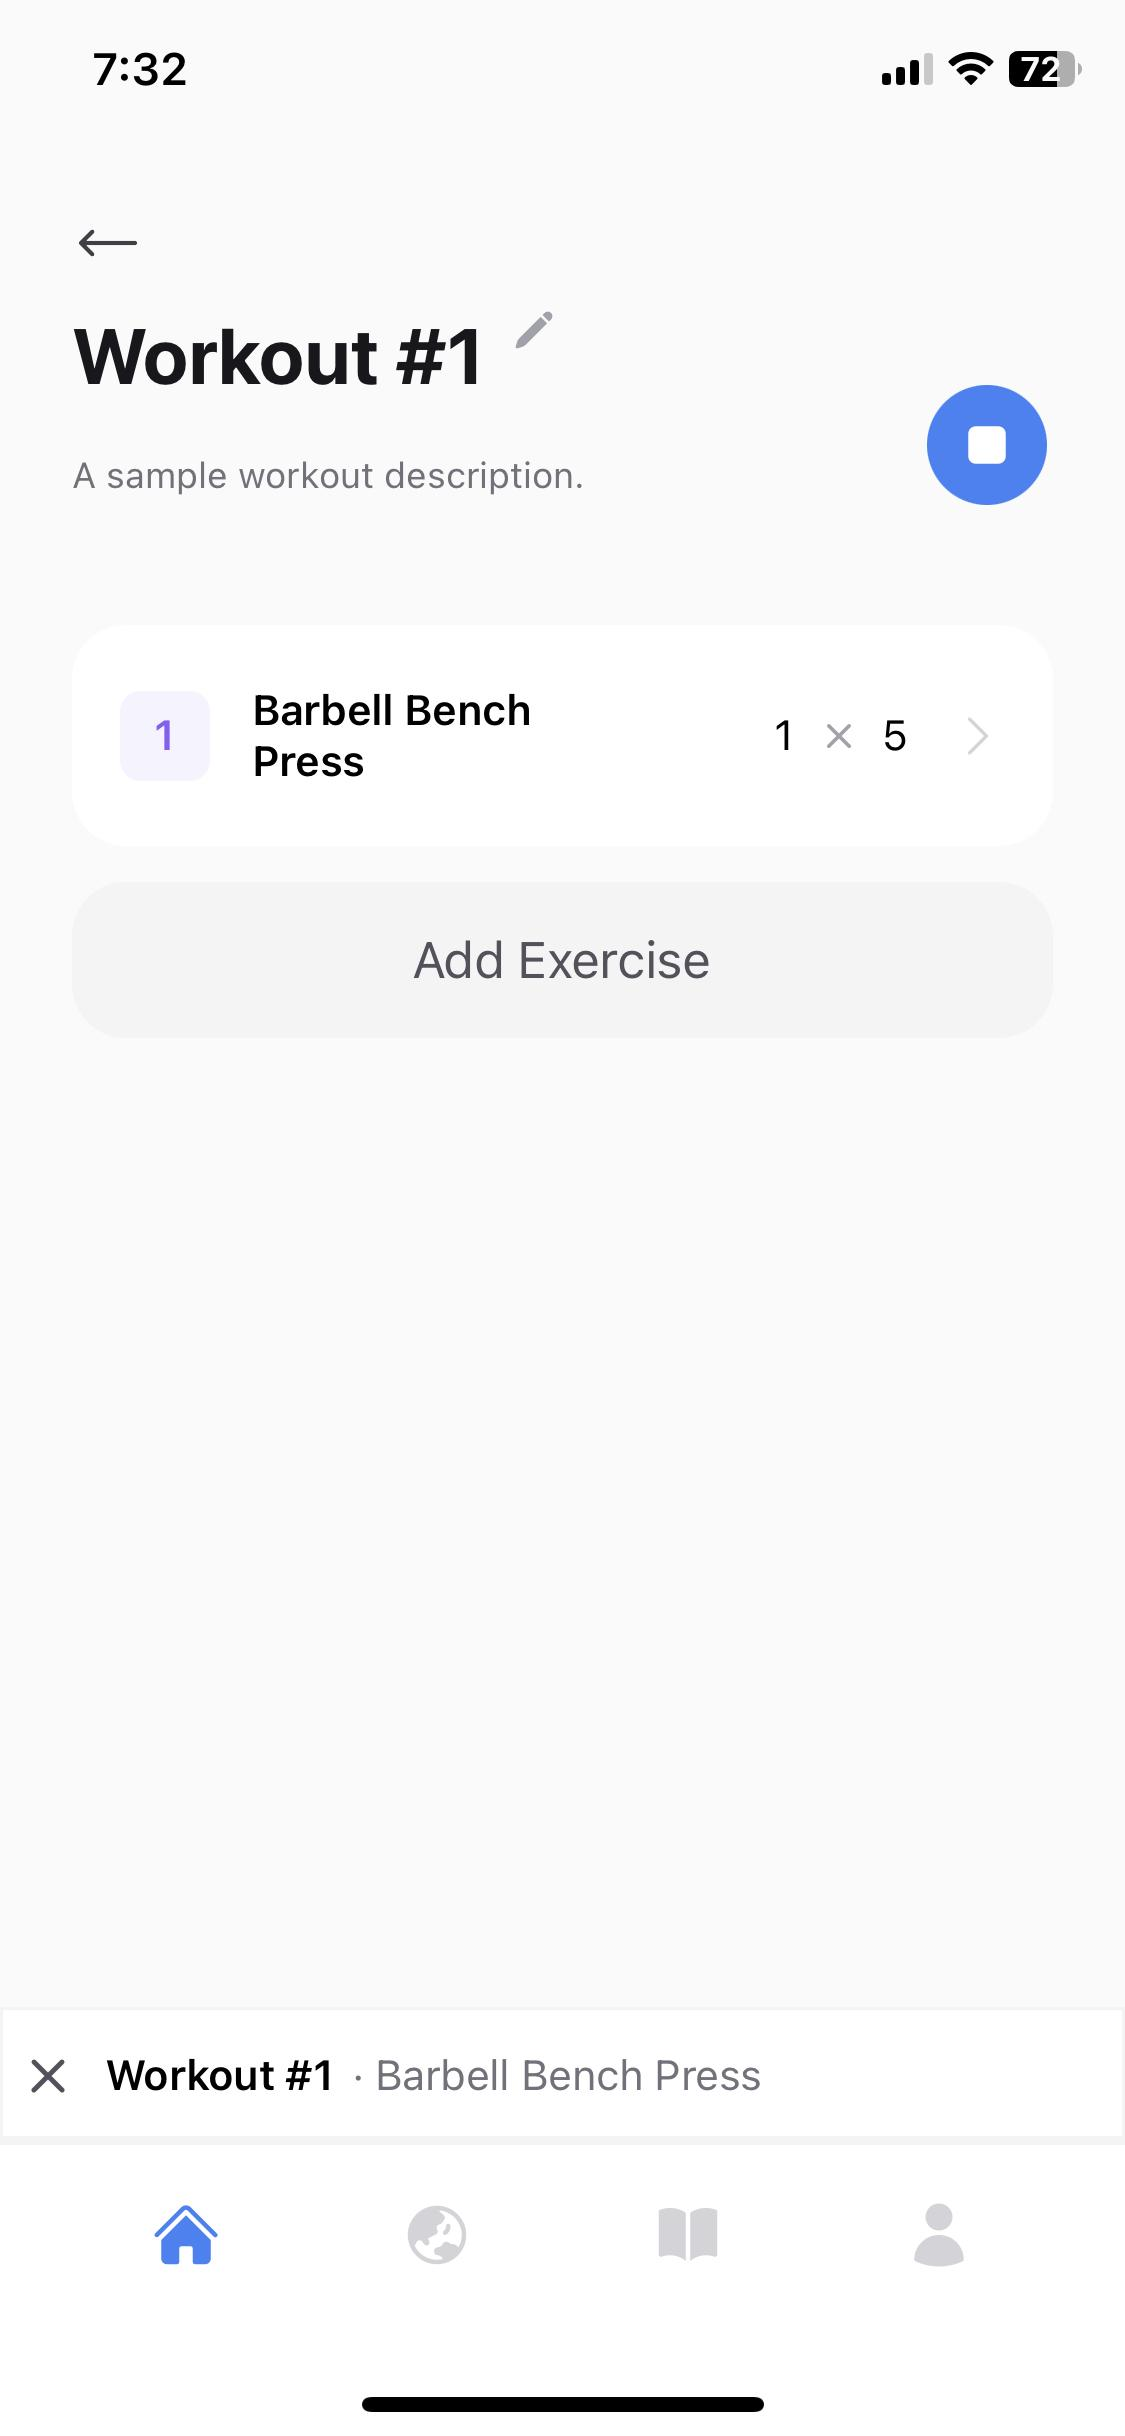
\includegraphics[height=0.6\textwidth]{imgs/ActiveWorkout.jpg}
    \caption{Edit Workout Screen}
    \label{FigEditWorkout}
    \end{figure}

\subsubsection{Exercise Addition}

When on the Add Exercise Page, users can select from a list of common exercises and add these to their workouts. Players will be able to customize the number of reps and rpes that should be achieved for each set. This is shown in Figure \ref{FigAddExercises}.

\begin{figure}[H]
    \centering
    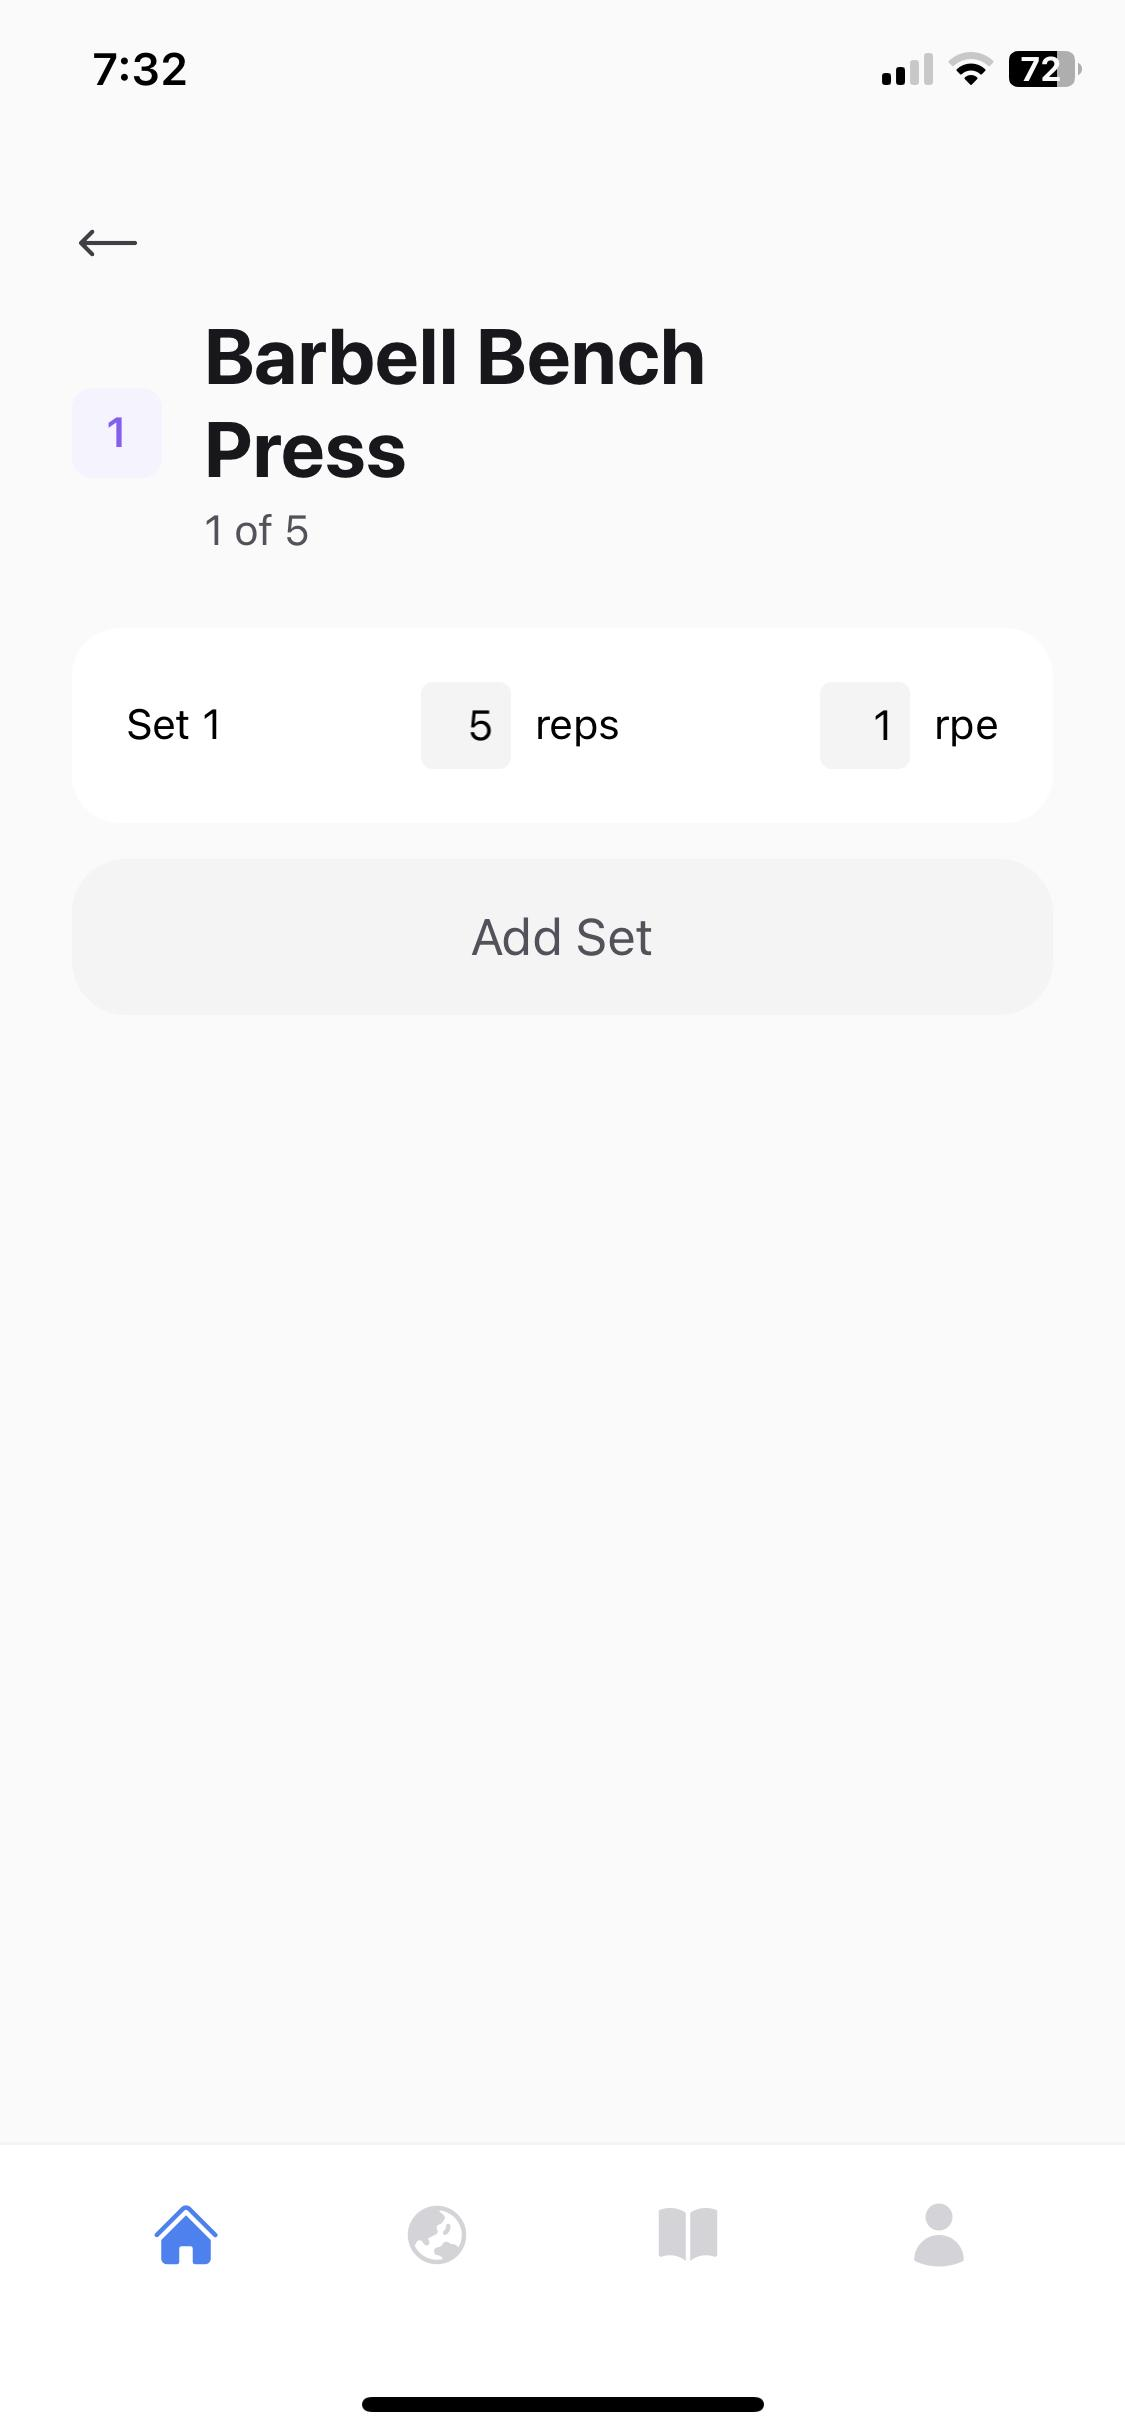
\includegraphics[height=0.6\textwidth]{imgs/SetExercise.jpg}
    \caption{Add Exercises Screen}
    \label{FigAddExercises}
    \end{figure}

\subsubsection{Program Discovery}

From the home page, press the Globe Icon on the bottom tab bar to visit the Discovery Page. From this page users can view popular programs by selecting tags as well as search for any Programs or Users.

\subsubsection{Programs View}

From the home page, press the Book Icon on the bottom tab bar to visit the Programs View. On this page users can view their existing Programs or return to the Create/Edit Program screen for individual programs by clicking on them.

\subsubsection{Profile}

From the home page, press the Avatar Icon on the bottom tab bar to visit the Profile Page. It can be seen in Figure \ref{FigProfile}.

\begin{figure}[H]
    \centering
    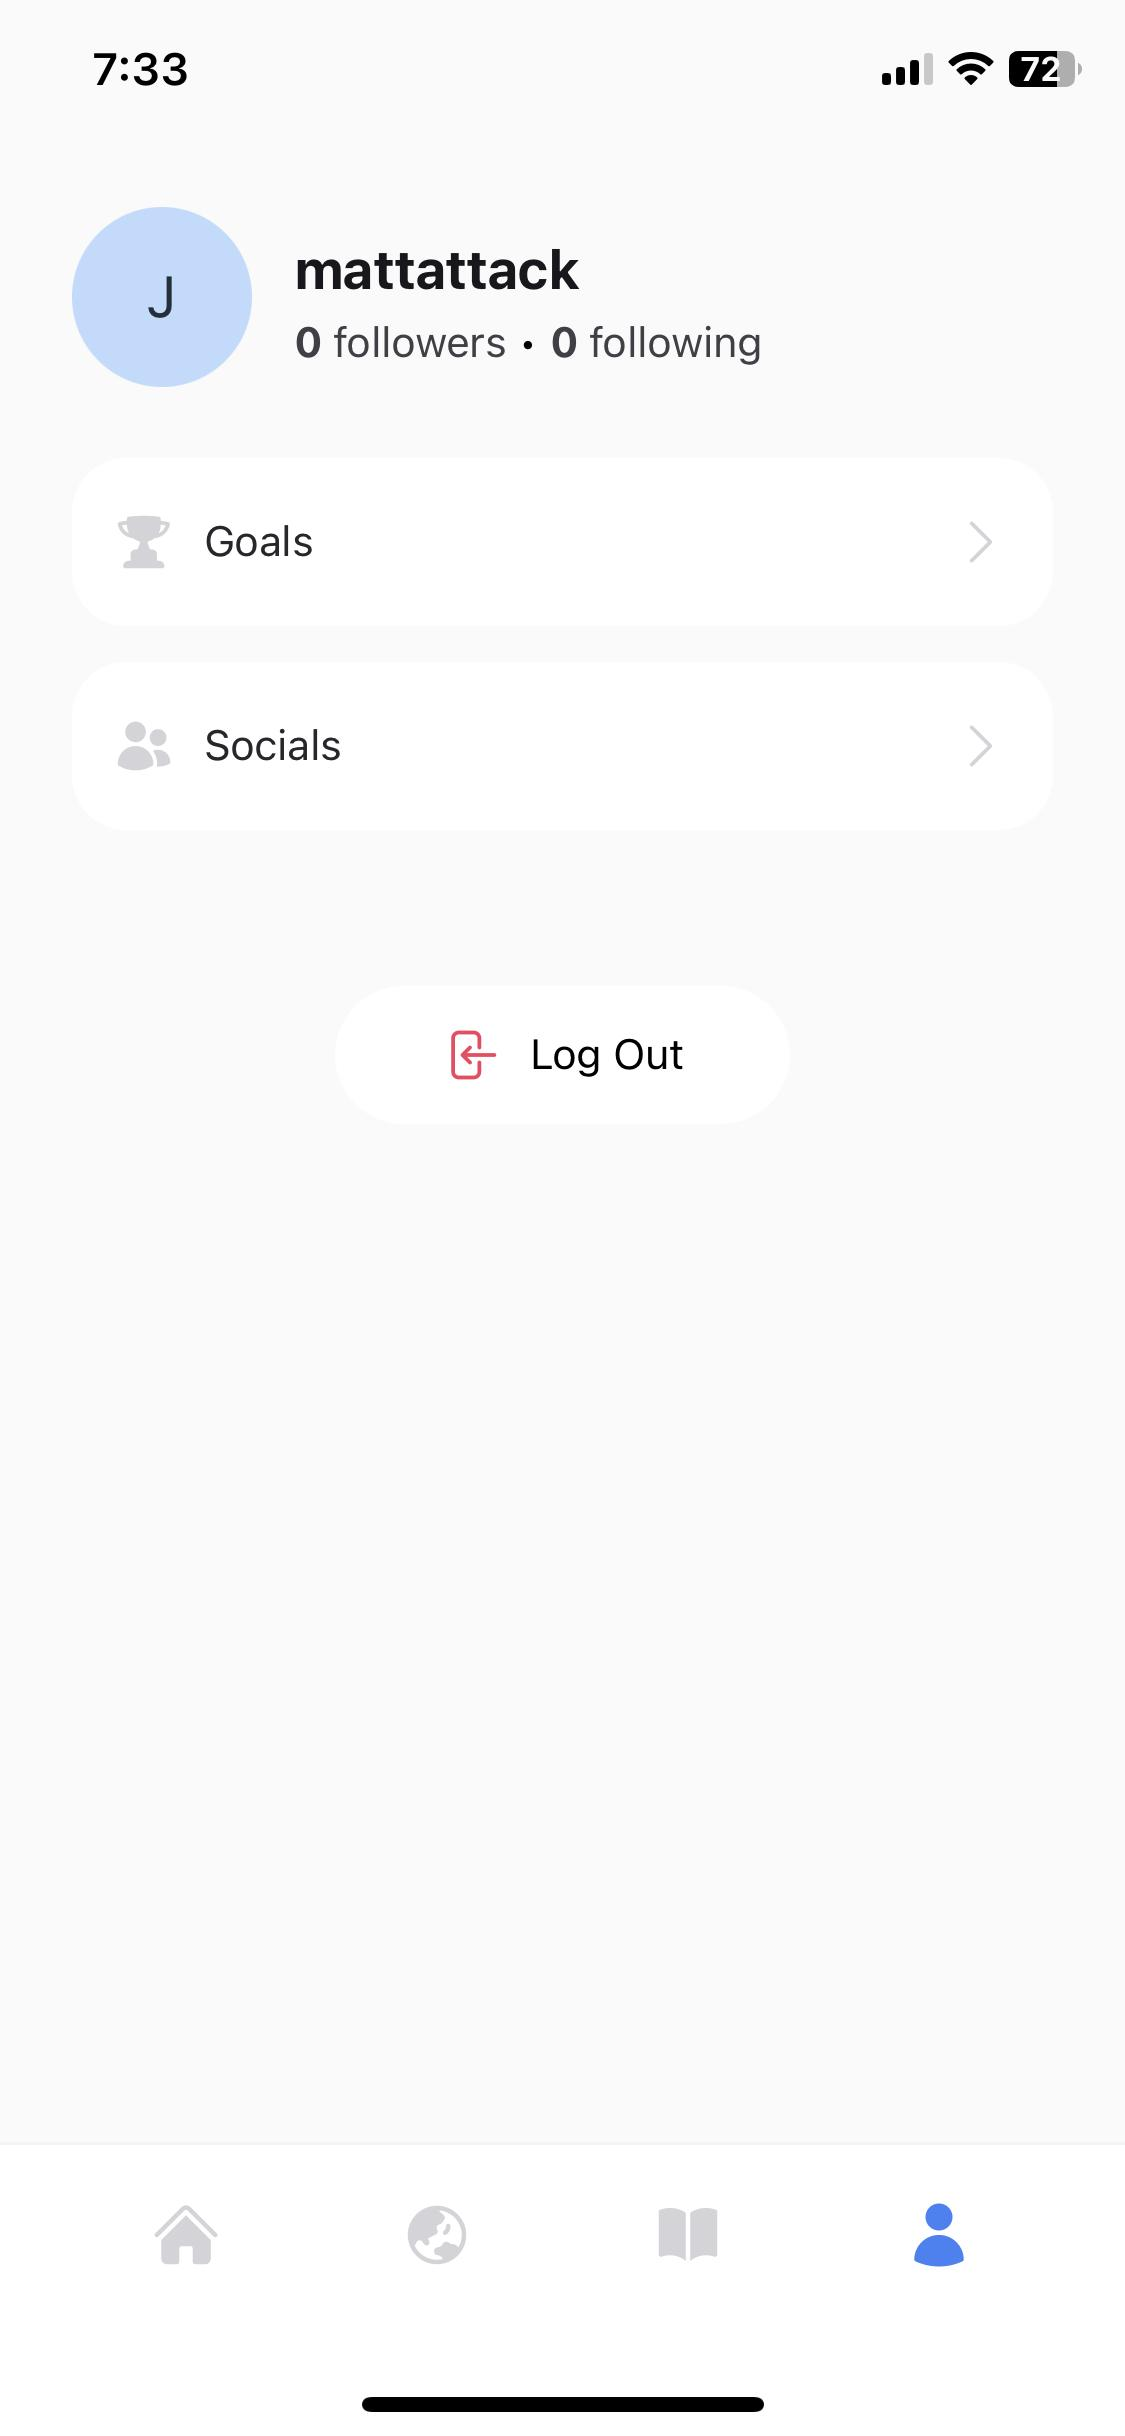
\includegraphics[height=0.6\textwidth]{imgs/Profile.jpg}
    \caption{Profile Screen}
    \label{FigProfile}
    \end{figure}

\subsubsection{Goals}

From the Profile Page, users can tap the "Goals" button to be redirected to the Goals page as shown in Figure \ref{FigGoals}. Users can use this page to set new goals and track existing ones. When setting goals users can set a weight and number of reps of a given exercise that they would like to work towards.

\begin{figure}[H]
    \centering
    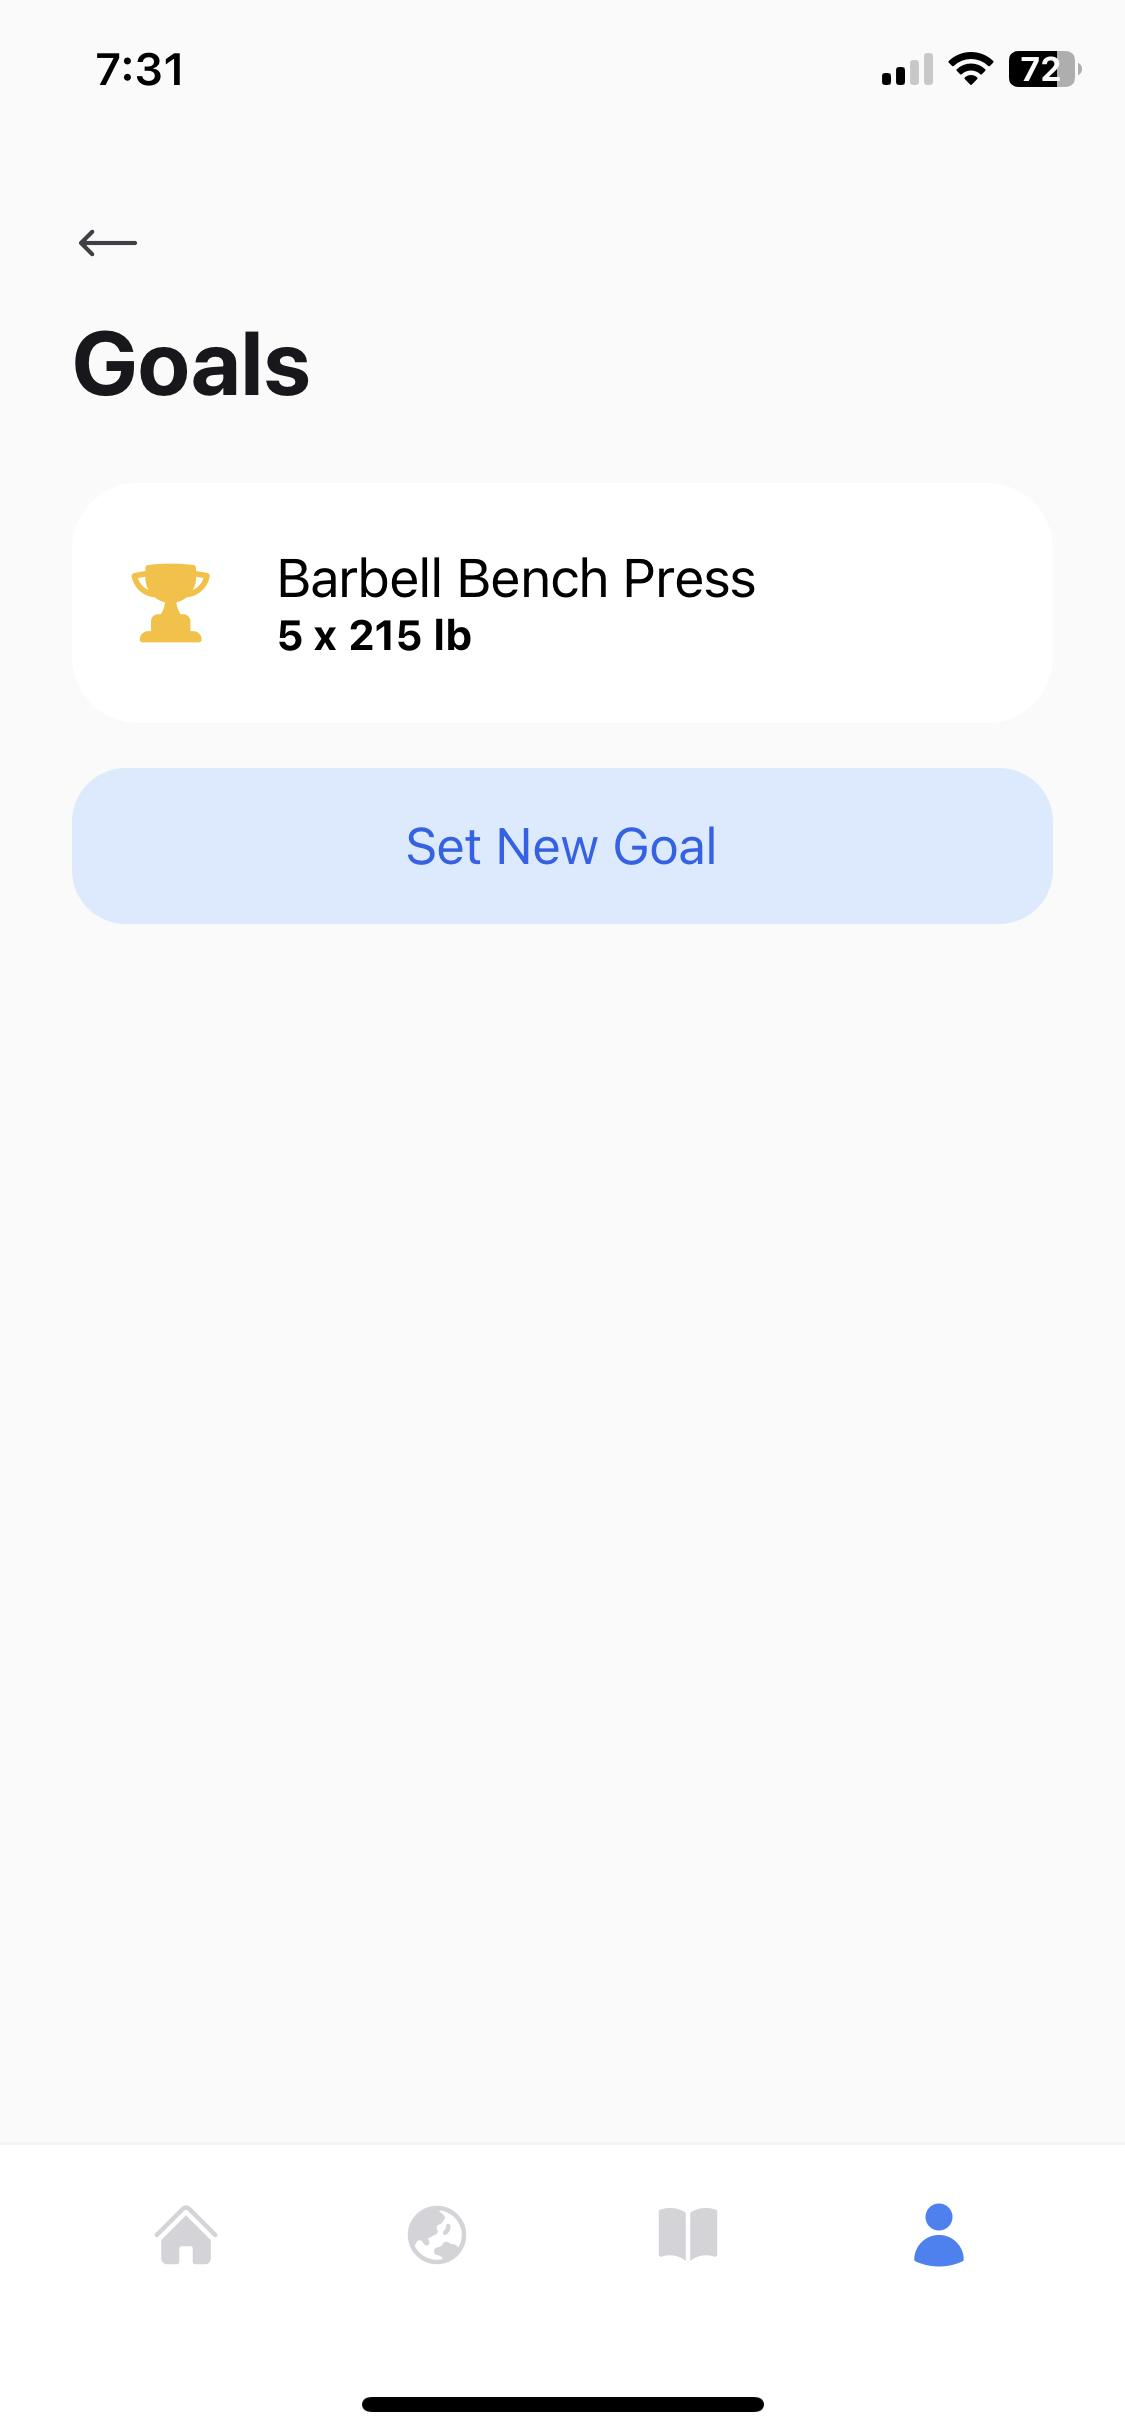
\includegraphics[height=0.6\textwidth]{imgs/Goals2.jpg}
    \caption{Goals Screen}
    \label{FigGoals}
    \end{figure}

\subsubsection{Socials}

From the Profile Page, users can tap the "Socials" button to be redirected to the Socials page. On this page they can view the Status of users that they follow and see any of their active workouts. Adding Followers will be covered in a future section.
    
\subsubsection{Adding Friends}

Users can add users by navigating to a users profile page in one of 2 ways:\\
\begin{enumerate}
    \item Search for a user on the Discover page in the search bar.
    \item Click on a users icon on any publicly visible workout that they created.
\end{enumerate}
Once on a users profile they can request to follow them.\\

\subsubsection{Start a Workout}

Users can start their workout by navigating to the Workout page as shown in Figure \ref{FigEditWorkout} and tapping the big blue play button. Once a workout is started, users can use the miniplayer at the bottom of the screen to progress their workout and check off completed exercises.

\end{document}